\chapter{Appendix: more papers}
\label{chapter:appendix}

%\minitoc
\chapterwithfigures{\nameref*{chapter:appendix}}
%\chapterwithtables{\nameref*{chapter:introduction}}

\ifthenelse{\boolean{skipAppendix}}{\endinput}{}

\section{Specific variations of Continual Learning}
\label{sec:related_variation}

While \acf{CIL}, detailed in \autoref{chapter:related}, is the most common benchmark in Continual
Learning, there are multiple variations of benchmark regardless which kind of shift is involved.

\subsection{Multiple labels}
\label{sec:related_multiple_labels}

The main task in Continual Learning is classification of a single class per sample, however it can
also be expanded to multiple classes per samples, \eg object detection
\citep{shmelkov2017incrementalobjectdetection} and semantic segmentation
\citep{michieli2019ilt,cermelli2020modelingthebackground}. The latter has seen recently interest
from the community for its concrete application: hand labeling in segmentation is extremely costly,
and continual segmentation propose to labelize only the new classes in an image, reducing greatly
the labeling cost. In that situation, a segmentation maps (made of one label per pixel) will only be
partially labelized: new classes are labelized, but old classes are assumed to be background.
Moreover, our model may have encountered new classes in the past, when they were themselves
considered as background. It's a case of concept shift, where the conditional distribution $p(y |
      x)$ changes through time. I detail in \autoref{chapter:segmentation} the existing benchmark in
\ac{CSS} and describe how we tackled this problem.

\subsection{Online Learning \& Task drift detection}
\label{sec:related_online_learning}

In Continual Learning, a model learns for multiple epochs for each task. On the other hand, in
Online Learning, also called Stream Learning, there are no notions of tasks nor epochs: a model must
learn on a stream of samples incoming one by one, and which cannot be replayed by epochs
\citep{aljundi2019notaskboundaries}. The methods to reduce forgetting described in
\autoref{sec:related_methods} can still be applied in Online Learning. Modified versions of
rehearsal learning, often inspired by reservoir sampling \citet{knuth97tacpvol2}, are often used
\citet{hayes2019exstream,aljundi2019taskfree}.

\begin{figure}[tb]
      \begin{center}
            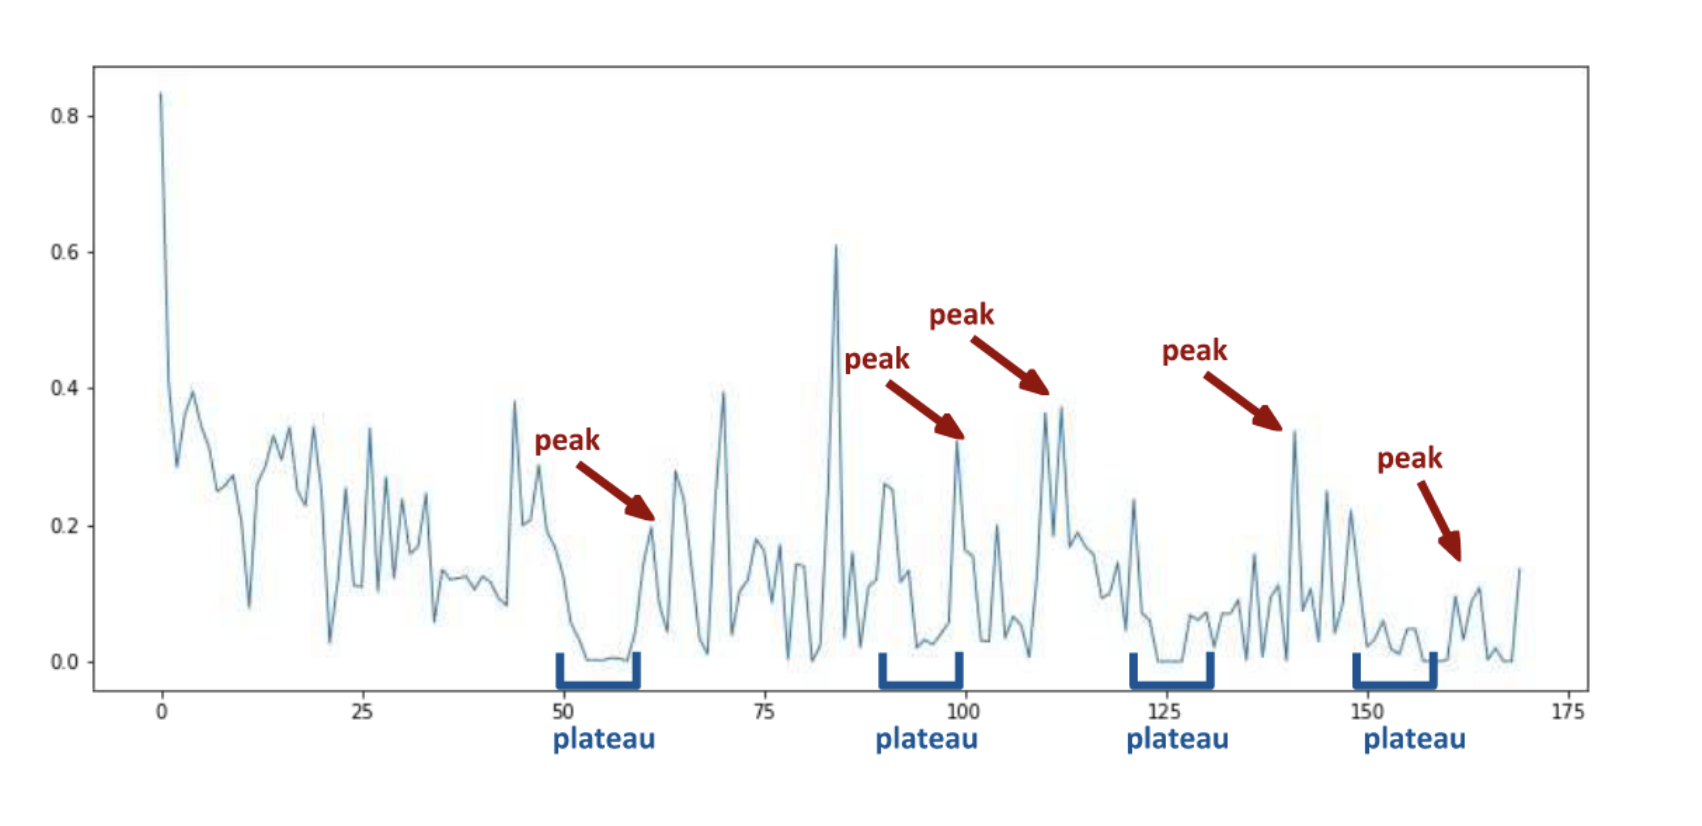
\includegraphics[width=0.6\linewidth]{images/related/loss_drift.png}
      \end{center}
      \caption{\textbf{Task-free detection of drift in the input distribution} by recording the
            plateau in the loss followed by a peak. y-axis is the loss value, and x-axis the update
            steps. Image from \citet{aljundi2019taskfree}.}
      \label{fig:related_lossdrift}
\end{figure}

Multiple regularization methods (\autoref{sec:related_regul}) needs to do some computation between
tasks. For example, weight-based regularization (\autoref{sec:related_regul_weight}) must compute
the task-specific importance weights. Because in Online Learning, there are no clear task
separation, a heuristic must determine when doing this computation. \citet{aljundi2019taskfree},
working a stream of images from soap operas, proposed to analyze the loss surface to find drift in
the distribution: at some point the model is experienced enough, and the loss starts to plateau.
When a drift happens, the loss will usually peak. This is a sign of task-free drift of the
distribution as illustrated in \autoref{fig:related_lossdrift}.

\subsection{Continual-Meta Learning}
\label{sec:related_meta}


Continual Learning aims to not forget. However, we --as humans-- often forget, but we can also
re-learn what was lost quicker than the first time. The goal of \ac{MCL} is therefore to recover as
quickly as possible --sample wise-- the original performance on past tasks
\citep{he2019metacontinual}. As the name implies, meta-learning methods, that aims to \textit{learn
      how to learn}, such as the MAML model \citep{finn2017maml} are used to that end. Then, \ac{MCL} has
been extended to a more general framework where the model also has to adapt quickly to new \acf{OoD}
tasks \citep{caccia2020osaka}.

Note that \acf{MCL} is not to be confused with \acf{CML} where in that case meta-learning is only
used during pretraining to provide better model initialization.

\subsection{Zeroshot Continual Learning}
\label{sec:related_zeroshot}


In Computer Vision, \acf{ZSL} \citep{lampert2009zeroshot,xian2019awa2} aims to classify classes that
were never seen before. To do so, models usually exploit an external knowledge source as a word2vec
embedding \citep{mikolov2013word2vec} trained on Wikipedia or an attribute matrix. Several works
have proposed to unify both Continual Learning and \ac{ZSL} where the future classes that haven't
been seen yet must be classified
\citet{lopezpaz2017gem,wei2020lifelongzeroshot,gautam2020continualzeroshot}. Rather than simply
using \ac{ZSL} as end to itself, we proposed, in \citep{douillard2020ghost}, to exploit its
properties to directly avoid forgetting. This is elaborated further in
\autoref{chapter:regularization} (\autoref{sec:ghost}).

\subsection{Natural Language Processing}
\label{sec:related_nlp}


Continual Learning can be applied to all modalities. After \acf{CV}, the most common one is
\ac{NLP}. \ac{NLP} saw its "\textit{ImageNet moment}" with the advent of Transformers
\citep{vaswani2017transformer}, and more recently with multi-tasks learning \citep{raffel2019t5}.
Continual \ac{NLP} \citet{biesialska2020continualnlp} aims naturally to learn multiple tasks, but in
a consecutive fashion with no --or few-- replay of the old tasks data. Applications can be similar
to \ac{CV} with addition of new classes \citep{masson2019episodiclifelongnlp} or new domains (\eg
medical corpus, fiction, tweets, etc.) \citep{gerald2021continualri}.

\subsection{Reinforcement Learning}
\label{sec:related_rl}


\ac{RL} \citep{sutton1998rl} more often than not needs support from Continual Learning
\citep{khetarpal2020continualrl}: for example as an agent evolves in an environment, it usually
needs rehearsal learning (also known as episodic memory) \citep{mnih2013atarirl}. Overall, the
methods originally developed for \ac{CV} (\autoref{sec:related_methods}) were then applied to both
\ac{NLP} and \ac{RL}.


\section{Details on PODNet}
\label{sec:appendix_podnet}

We also compared our model against baselines with a more flexible memory $M_{\text{total}} = 2000$
\citep{rebuffi2017icarl,wu2019bias_correction}, and with various initial task size (by default it is
50 on CIFAR100). In the former case (\autoref{tab:podnet_sub_free_memory}), models benefit from a
larger memory per class in the early tasks. In the later case
(\autoref{tab:podnet_sub_initialincrement}), models initialization is worse because of a smaller
initial task size. In these settings very different from \autoref{sec:podnet_quantitative_results},
\ac{PODNet} still outperformed significantly the compared models, proving the robustness of our
model.

\begin{table*}
    \centering
    \begin{tabular}{@{}l|cc@{}}
        \toprule
                                                            & \multicolumn{2}{c}{Nb. steps}                  \\
        \cmidrule{2-3}
        Loss                                                & 50                            & 10             \\
        \midrule
        iCaRL \citep{rebuffi2017icarl}                      & 42.34                         & 56.52          \\
        BiC \citep{wu2019bias_correction}                   & 48.44                         & 55.03          \\
        UCIR\,{\scriptsize (\ac{NME})}\,\citep{hou2019ucir} & 54.08                         & 62.89          \\
        UCIR\,{\scriptsize (CNN)}\,                         & 55.20                         & 63.62          \\
        PODNet\,{\scriptsize (\ac{NME})}                    & \textbf{62.47}                & \textbf{64.60} \\
        PODNet\,{\scriptsize (CNN)}                         & \textbf{61.87}                & \textbf{64.68} \\
        \bottomrule
    \end{tabular}
    \caption{\textbf{Evaluation of an easier memory constraint:} ($M_\mathrm{total} = 2000$)}
    \label{tab:podnet_sub_free_memory}
\end{table*}

\begin{table*}
    \centering
    \begin{tabular}{@{}l|ccccc@{}}
        \toprule
                                                                        & \multicolumn{5}{c}{Initial task size}                                                                     \\
        \cmidrule{2-6}
        Loss                                                            & 10                                    & 20             & 30             & 40             & \textbf{50}    \\
        \midrule
        iCaRL \scriptsize{\citep{rebuffi2017icarl}}                     & 40.97                                 & 41.28          & 43.38          & 44.35          & 44.20          \\
        BiC \scriptsize{\citep{wu2019bias_correction}}                  & 41.58                                 & 40.95          & 42.27          & 45.18          & 47.09          \\
        UCIR\,{\scriptsize (\ac{NME})} \scriptsize{\citep{hou2019ucir}} & 42.33                                 & 40.81          & 46.80          & 46.71          & 48.57          \\
        UCIR\,{\scriptsize (CNN)}                                       & 43.25                                 & 41.69          & 47.85          & 47.51          & 49.30          \\
        PODNet\,{\scriptsize (\ac{NME})}                                & \textbf{45.09}                        & \textbf{49.03} & \textbf{55.30} & \textbf{57.89} & \textbf{61.40} \\
        PODNet\,{\scriptsize (CNN)}                                     & \textbf{44.95}                        & \textbf{47.68} & \textbf{52.88} & \textbf{55.42} & \textbf{57.98} \\
        \bottomrule
    \end{tabular}
    \caption{\textbf{Varying initial task size:} with $M_\mathrm{per} = 20$, and followed by 50 to 90 tasks made of a single class.}
    \label{tab:podnet_sub_initialincrement}
\end{table*}


\subsection{Implementation details}

For all datasets, images are augmented with random crops and flips. For CIFAR100, we additionally
change image intensity by a random value in the range [-63, 63].
%
We train our model for 160 epochs for CIFAR100, and 90 epochs for both ImageNet100 and ImageNet100,
with a SGD optimizer with momentum of 0.9. For all datasets, we start with a learning rate of 0.1, a
batch size of 128, and cosine annealing scheduling.
%
The weight decay is $5\cdot 10^{-4}$ for CIFAR100, and $1\cdot 10^{-4}$ for ImageNet100 and
ImageNet1000. For CIFAR100 we set model hyperparameters $\lambda_c = 3$ and $\lambda_f=1$, while for
ImageNet100 and 1000 we set $\lambda_c = 8$ and $\lambda_f =10$. Our model uses POD-spatial and
POD-flat except when explicitly stated otherwise. Following \citet{hou2019ucir}, we multiply both
losses by the adaptive scaling factor: $\lambda=\sqrt{\nicefrac{N}{T}}$ with $N$ being the number of
seen classes and $T$ the number of classes in the current task.

For POD-spatial, before sum-pooling we take the features to the power of 2 element-wise. The vector
resulting from the pooling is then L2 normalized.

\subsection{Number of proxies per class}

While our model's expressiveness increases with more proxies in $\mcL_\text{LSC}$, it remains fairly
stable for values between 5 and 15, thus, for simplicity, we kept it fixed to 10 in all experiments.

In initial experiments, we had the following pairs for the number of clusters (k) and average
incremental accuracy (acc): k=1, acc=56.80\%; k=2, 57.14\%; k=4, acc=57.40\%; k=6, acc=57.46\%; k=8,
acc=57.95\%, and k=10, acc=57.98\% --- i.e., a 1.18 p.p. improvement moving from k=1 to k=10. On
ImageNet100, with 10 steps/tasks (increments of give classes per task), moving from k=1 to k=10
improved 1.51 p.p. on acc.

\subsection{Reproducibility}

\paragraph{Code Dependencies} The Python version is  3.7.6. We used the PyTorch
\citep{paszke2017pytorch} (version 1.2.0) deep learning framework and the libraries Torchvision
(version 0.4.0), NumPy \citep{oliphant2006numpy} (version 1.17.2), Pillow (version 6.2.1), and
Matplotlib \citep{hunter2007matplotlib} (version 3.1.0). The CUDA version is 10.2. Initial
experiments were done with the data loaders library Continuum \citep{douillardlesort2020continuum}.
PODNet's full code is released at:\\
\href{https://github.com/arthurdouillard/incremental\_learning.pytorch}{\texttt{github.com/arthurdouillard/incremental\_learning.pytorch}}.
\\We provide all configuration files necessary to reproduce results, including seeds and class
ordering.

\paragraph{Datasets description} I provide bellow extensive details on the content of the three
datasets considered for PODNet: CIFAR100, ImageNet100, and ImageNet1000.

{\begin{description} \setlength{\parskip}{0pt}
      \item[CIFAR100] contains 32$\times$32-pixel images in 100 classes, with 50k images for
            training and 10k for testing.
      \item[ImageNet100] contains 224$\times$224-pixel images in 100 classes, with $\sim$128k images
            for training and $\sim$5k for testing.
      \item[ImageNet1000] contains 224$\times$224-pixel images in 1000 classes, with $\sim$1.28m
            images for training and $\sim$50k for testing. \end{description}}

\paragraph{Spatial-based distillation} I displayed the differences of performance between
spatial-based distillation in \autoref{sec:podnet_ablation_pooling}
(\autoref{tab:podnet_ablation_perceptual}) when combined with POD-flat. In this appendix, I also
detail in \autoref{tab:podnet_ablation_perceptual_noflat} the same spatial-loss without POD-flat.
The ranking between distillation losses is ostensibly the same. Notice that POD-spatial ---and its
sub-components POD-width and POD-height-- are the only losses barely affected by POD-flat's absence.
Note that all alternative losses were tuned on the validation set to get the best performance,
including those from external papers. Still, our proposed loss, POD-spatial, outperforms all, both
with and without POD-flat.


\begin{table*}[!htbp]
    \centering
    \begin{tabular}{@{}lcc@{}}
        \toprule
        Loss                                                        & NME            & CNN            \\
        \midrule
        \textit{None}                                               & 41.56          & 40.76          \\
        POD-pixels                                                  & 42.21          & 40.81          \\
        POD-channels                                                & 55.91          & 50.34          \\
        POD-gap                                                     & 57.25          & 53.87          \\
        POD-width                                                   & 61.25          & 57.51          \\
        POD-height                                                  & 61.24          & 57.50          \\
        POD-spatial                                                 & \textbf{61.42} & \textbf{57.64} \\
        \hdashline
        GradCam~\citep{dhar2019learning_without_memorizing_gradcam} & 41.89          & 42.07          \\
        Perceptual Style~\citep{johnson2016perceptual_losses}       & 41.74          & 40.80          \\
        \bottomrule
    \end{tabular}
    \caption{\textbf{Comparison of distillation losses} based on intermediary features. All losses evaluated
        without POD-flat. We report the average incremental accuracy on CIFAR100 with 50 steps.}
    \label{tab:podnet_ablation_perceptual_noflat}
\end{table*}



\section{Details on Ghost}
\label{sec:appendix_ghost}


\subsection{Overhead of SVMs training}

Training the SVMs for $\mcL^{\text{\tiny{svm-reg}}}$ introduces a computational overhead. To
minimize it, we limit the number of features per class to 500. Moreover, as we advance towards later
tasks, fewer unseen classes remain, and thus we have fewer SVMs to train. Overall, an experiment on
AwA2, with our setting of 25 classes + 5 $\times$ 5 classes, takes 5 hours to train. We observed
that our SVM-based regularization extends that time by less than 5 minutes on average, an overhead
of less than 2\%, which we deemed acceptable. For reference, the SVMs were trained on a machine with
10 CPU cores of 3.90GHz each.

\subsection{Implementation Details} For all datasets and settings, we set the classification margin
$\delta=0.6$, and the SVM latent-space regularization additional margin $\tau=1$. We train the
feature-extractor-and-classifier pipeline for 90 epochs with an SGD optimizer, learning rate of 0.1,
cosine scheduling, and weight decay of $10^{-4}$. We train the generator for 1200 epochs, with an
Adam optimizer and a learning rate of $10^{-5}$. Finally, following
\citet{hou2019ucir,douillard2020podnet}, we fine-tune the classifier for 60 epochs (with the feature
extractor frozen and a small learning rate of $10^-4$) at the end of every task (except the last
one). We found useful to balance the bias towards the seen classes against the unseen classes. With
the POD distillation \citet{douillard2020podnet}, we set $\lambda_1=3$  for AwA2, and $\lambda_1=15$
for aP\&Y; with the Less-Forget distillation \citet{hou2019ucir}, we set $\lambda_1=4$ for both
datasets. We always set $\lambda_2=10^{-3}$, moreover we apply it on L2-normalized features.
Finally, we do not reinitialize the models between tasks: $f^t$ results from training $f^{t-1}$ on
task $t$, etc. On the rehearsal memory limitation, we follow the strict setting of Hou et
al.~\citet{hou2019ucir}, keeping only $s=20$ training images per past class.

\subsection{Datasets details}

We train our model on three datasets: MNIST, AwA2, and aP\&Y. Baselines and our Ghost models are run
on the exact same data/class splits, with the exact same preprocessing.

\paragraph{MNIST} This dataset has ten classes: handwritten digits ranging from '0'' to '9'. It has
a training set of 60,000 images and a test set of 10,000 images. We used for validation set, a
subset of 10,000 examples of the training set. Images are in black\&white (one channel) and of
dimension $28\times28$. We convert the pixels values to the range [0, 1] and then normalize by the
mean and standard deviation of the training dataset.

\paragraph{AwA2} This dataset has 50 animals classes. It has a training set of 29,857 images and a
test set of 7,465 images. We used for validation set a subset of 8,000 images of the training set.
Images are in RGB color. We convert the pixel values to the range [0, 1] and normalize by the mean
and standard deviation of the training dataset. Train images are randomly cropped to a square of
$224\times224$ and are randomly flipped horizontally. Test images are resized to $256\times256$ and
then center cropped to $224\times224$.

\paragraph{aP\&Y} This dataset has 32 classes of everyday objects. It has a training set of 12,269
images and a test set of 3,068 images. We used for validation set a subset of 4,000 images of the
training set. Images are in RGB color. We convert the pixel values to the range [0, 1] and normalize
by the mean and standard deviation of the training dataset. Train images are randomly cropped to a
square of $224\times224$ and are randomly flipped horizontally. Test images are resized to
$256\times256$ and then center cropped to $224\times224$.

\subsection{Reproducibility}

\paragraph{Code Dependencies} The Python version is  3.7.6. We used the PyTorch
\citet{paszke2017pytorch} (version 1.2.0) deep learning framework and the libraries Torchvision
(version 0.4.0), NumPy \citet{oliphant2006numpy} (version 1.17.2), Pillow (version 6.2.1), and
Matplotlib \citet{hunter2007matplotlib} (version 3.1.0). The CUDA version is 10.2. Experiments on
MNIST were done with the data loaders library Continuum \citet{douillardlesort2021continuum}.

The code is released at
\href{https://github.com/arthurdouillard/incremental_learning.pytorch}{github.com/arthurdouillard/incremental\_learning.pytorch}.

\paragraph{Hardware \& Training duration} We ran our experiments on 3 Titan Xp GPUs with 12 Go of
VRAM each. Each experiment had access to 10 CPU cores of 3.90 GHz each, and used at most 3 Go of RAM
and 8 Go of VRAM. A single experiment run on AwA2 took on average 5 hours and, on aP\&Y, 3 hours. We
ran each experiment thrice with different random seeds (1, 2, and 3).


\section{Details on DyTox}
\label{sec:appendix_dytox}


\noindent\autoref{tab:dytox_notation} summarizes the notations used along this paper.

\begin{table}[t]
    \centering
    \begin{tabular}{@{}l|l@{}}
        \hline
        Symbol                 & Meaning\Tstrut\Bstrut                                   \\
        \hline
        $(x_i^t, y_i^t)$       & Input sample \& its label from the $t^{th}$ task\Tstrut \\
        $C^t$                  & Label set of the $t^{th}$ task                          \\
        $C^{1:t}$              & All labels from all seen tasks                          \\
        $\theta_t$             & Task token of the $t^{th}$ task                         \\
        $\operatorname{Clf}_t$ & Independent classifier of the $t^{th}$ task             \\
        $\operatorname{SAB}_l$ & $l^{th}$ Self-Attention Block                           \\
        $\operatorname{TAB}$   & Task-Attention Block                                    \\
        \hline
    \end{tabular}
    \caption{\textbf{Notations} used in the paper.}
    \label{tab:dytox_notation}
\end{table}



\subsection{Experimental details}

\paragraph{Datasets} We use three datasets: CIFAR100 \citep{krizhevskycifar100}, ImageNet100, and
ImageNet1000 \citep{deng2009imagenet}. CIFAR100 is made of 50,000 train RGB images and 10,000 test
RGB images of size $32\times32$ for 100 classes. ImageNet1000 contains 1.2 million RGB train images
and 50,000 validation RGB images of size $224\times224$ for 1000 classes. ImageNet100 is a subset of
100 classes from ImageNet1000. We follow PODNet \citep{douillard2020podnet} and DER \citep{yan2021der}
and use the same 100 classes they've used. Fine details about the datasets, like the class orders,
can be found in the provided code in the options files (see readme).

\paragraph{Implementation} For all datasets, we train the model for 500 epochs per task with Adam
\citep{kingma2014adam} with a learning rate of $5e^{-4}$, including 5 epochs of warmup.
Following UCIR \citep{hou2019ucir}, PODNet \citep{douillard2020podnet}, and DER \citep{yan2021der}, at
the end of each task (except the first) we finetuned our model for 20 epochs with a learning rate of
$5e^{-5}$ on a balanced dataset. In DyTox, we applied the standard data augmentation of DeiT
\citep{touvron2021deit} but we removed the pixel erasing \citep{zhong2017erasing}, MixUp
\citep{hingyi2018mixup}, and CutMix \citep{yun2019cutmix} augmentations for fair comparison. In
contrast, in DyTox+ we used a MixUp \citep{hingyi2018mixup} with beta distribution $\beta(0.8, 0.8)$.
During all incremental tasks ($t>1$), the old classifiers $\operatorname{Clf}_i,\, i < t$ and the
old task tokens $\theta_i,\, i < t$ parameters are frozen. During the finetuning phase where classes
are rebalanced \citep{castro2018end_to_end_inc_learn,hou2019ucir,douillard2020podnet,yan2021der},
these parameters are optimized, but the SABs are frozen.

\paragraph{Hyperparameter tuning} In contrast with previous works
\citep{douillard2020podnet,yan2021der}, we wanted stable hyperparameters, tuned for a single setting
and then applied on all experiments. This avoids optimizing for the number of tasks, which defeats
the purpose of continual learning \citep{farquhar2018robustcontinual}. We tuned hyperparameters for
DyTox using a validation subset made of 10\% of the training dataset, and this only on the CIFAR100
experiment with 10 steps. We provide in \autoref{tab:dytox_tuning} the chosen hyperparameters. Results in
the main paper shows that those hyperparameters reach state-of-the-art on all other settings and
notably on ImageNet.

\begin{table}[t]
    \centering
    \resizebox{\textwidth}{!}{%
        \begin{tabular}{l|cc}
            \hline
            Hyperparameter        & Range                           & Chosen value\Tstrut\Bstrut \\
            \hline
            Learning rate         & $1e^{-3}$, $5e^{-4}$, $1e^{-4}$ & $5e^{-4}$\Tstrut           \\
            Epochs                & 300, 500, 700                   & 500                        \\
            $\lambda$             & 0.05, 0.1, 0.5                  & 0.1                        \\
            CIFAR's patch size    & 4, 8, 16                        & 4                          \\
            ImageNet's patch size & 14, 16                          & 16                         \\
            \hline
        \end{tabular}
    }
    \caption{\textbf{Hyperparameters} that were tuned from the codebase of \cite{touvron2021deit}.
        We ran a gridsearch on CIFAR100 10 steps on a validation set made of 10\% of the training set,
        and kept fixed the chosen hyperparameters for all experiments (any number of steps and any
        datasets).}
    \label{tab:dytox_tuning}
\end{table}


\paragraph{Baselines} E2E \citep{castro2018end_to_end_inc_learn} and Simple-DER \citep{li2021preserve}
results come from their respective papers. All other baseline results are taken from the DER paper
\citep{yan2021der}. We now further describe their contributions. iCaRL \citep{rebuffi2017icarl} uses a
knowledge distillation loss \citep{hinton2015knowledge_distillation} and at test-time predicts using
a k-NN from its features space. E2E \citep{castro2018end_to_end_inc_learn} learns a model with
knowledge distillation and applies a finetuning after each step. UCIR \citep{hou2019ucir} uses cosine
classifier and euclidean distance between the final flattened features as a distillation loss. BiC
\citep{wu2019bias_correction} uses a knowledge distillation loss and also re-calibrates
\citep{guo2017miscalibration} the logits of the new classes using a simple linear model trained on
validation data. WA \citep{zhao2020weightalignement} uses a knowledge distillation loss and
re-weights at each epoch the classifier weights associated to new classes so that they have the same
average norm as the classifier weights of the old classes. PODNet \citep{douillard2020podnet} uses a
cosine classifier and a specific distillation loss (POD) applied at multiple intermediary features
of the ResNet backbone. RPSNet \citep{rajasegaran2019rpsnet} uses knowledge distillation and
manipulates subnetworks in its architecture, following the lottery ticket hypothesis
\citep{frankle2019lottery_ticket}. DER \citep{yan2021der} creates a new ResNet per task. All ResNets'
embeddings are concatenated and fed to a unique classifier. ResNets are pruned using HAT
\citep{serra2018hat} masking procedure. Note that DER pruning has multiple hyperparameters that are
set differently according to the settings. Furthermore, the reported parameters count, after
pruning, in \citep{yan2021der} is an average of the count over all steps: the final parameters count
(necessarily higher) wasn't available. Finally, Simple-DER \citep{li2021preserve} is similar to DER,
with a simpler pruning method which doesn't require any hyperparameter tuning.

\begin{table}[t]
    \centering
    \begin{tabular}{@{}c|ccc@{}}
        \hline
        \textbf{TAB parameter sharing?} & \textbf{\#P} & \textbf{Avg} & \textbf{Last}\Tstrut\Bstrut \\
        \hline
        %Param-free TAB & 10,11 & 67.61 & 49.16\\
        %TAB noMLP & 10,25 & 68.50 & 50.29 \\
        %Single TAB forward & 10.77 & 67.78 & 48.73 \\
        %Only Query & 10.77 & 67.79 & 49.53\\
        %TAB Batch Ensemble \cite{wen2020batchensemble} & 10,81 & 68.42 & 49.54 \\
        \xmark                          & 97.59        & 72.20        & 56.00                       \\
        %5 SABs + 2 TABs & 12.48 & 70.35 & 52.69\\
        %4 SABs + 2 TAB & 10.77 & 70.29 & 52.37 \\

        \cmark                          & 10.77        & 70.20        & 52.34                       \\
        \hline
    \end{tabular}
    \caption{\textbf{Investigation of the parameter sharing of TAB}. We report the ``Avg'' accuracy
        and the ``Last'' accuracy for the 50 steps setting on CIFAR100. The second row corresponds to
        DyTox.}
    \label{tab:dytox_alternatives}
\end{table}



%\begin{table*}[t]
    \centering
    \resizebox{1.0\textwidth}{!}{%
        \begin{tabular}{@{}l|ccc|ccc|ccc}
            \hline
                                                & \multicolumn{3}{c|}{10 steps} & \multicolumn{3}{c|}{20 steps} & \multicolumn{3}{c}{50 steps}                                                                                                                                              \\
            \textbf{Methods}                    & \textbf{\#P}                  & \textbf{Avg}                  & \textbf{Last}                & \textbf{\#P} & \textbf{Avg}                & \textbf{Last}               & \textbf{\#P} & \textbf{Avg}                & \textbf{Last}      \\
            \hline
            ResNet18 Joint                      & 11.22                         & -                             & 80.41                        & 11.22        & -                           & 81.49                       & 11.22        & -                           & 81.74              \\
            Transf. Joint                       & 10.72                         & -                             & 76.12                        & 10.72        & -                           & 76.12                       & 10.72        & -                           & 76.12              \\
            \hline
            WA \cite{zhao2020weightalignement}  & 11.22                         & 69.46\scriptsize{\mypm0.29}   & 53.78                        & 11.22        & 67.33\scriptsize{\mypm0.15} & 47.31                       & 11.22        & 64.32\scriptsize{\mypm0.28} & 42.14              \\
            DER \small{w/o P} \cite{yan2021der} & 112.27                        & 75.36\scriptsize{\mypm0.36}   & \textbf{65.22}               & 224.55       & 74.09\scriptsize{\mypm0.33} & \textbf{62.48}              & 561.39       & 72.41\scriptsize{\mypm0.36} & \textbf{59.08}     \\ % no pruning
            \hline
            DyTox                               & 10.73                         & 73.66\mysmpm{0.02}            & 60.67\mysmpm{0.34}           & 10.74        & 72.27\mysmpm{0.18}          & 56.32\mysmpm{{0.61}}        & 10.77        & 70.20\mysmpm{0.16}          & 52.34\mysmpm{0.26} \\
            DyTox+                              & 10.73                         & 75.54\mysmpm{0.10}            & 62.06\mysmpm{0.25}           & 10.74        & 75.04\mysmpm{0.11}          & 60.03\mysmpm{0.45}          & 10.77        & 74.35\mysmpm{0.05}          & 57.09\mysmpm{0.13} \\
            DyTox++                             & 10.73                         & \textbf{77.10\mysmpm{0.08}}   & 64.53\mysmpm{0.08}           & 10.74        & \textbf{76.57\mysmpm{0.18}} & \textbf{62.44\mysmpm{0.22}} & 10.77        & \textbf{75.45\mysmpm{0.19}} & 58.76\mysmpm{0.28} \\
            \hline
        \end{tabular}}
    \caption{\textbf{Results on CIFAR100} averaged over three different class orders. WA and DER w/o
        P results are reported from \cite{yan2021der}. DyTox+ uses MixUp in addition of the DyTox
        strategy, DyTox++ further adds a sharpness-aware minimization \cite{kwon2021asam}.}
    \label{tab:dytox_cifar100-b0_pp}
\end{table*}


\subsection{Parameter sharing of the TAB}

Previous dynamic methods as DER \citep{yan2021der} and Simple-DER \citep{li2021preserve} shared no
parameters between tasks until the final classifier. We proposed instead with DyTox to share the
encoder (SABs) and the decoder (TAB) parameters across tasks, leading to a minimal memory overhead
while also sharing common information between tasks. In \autoref{tab:dytox_alternatives}, we compare the
impact of sharing the TAB per task --- and only maintain different tokens per task. In the first
row, a different TAB is created per task, while in the second row the same TAB is used --- which is
the DyTox strategy. A different TAB per task leads to better results (56\% \textit{v.s.} 52\% in
``Last'' accuracy) because the network can be more diverse with each TAB specialized to its
associated task. This increased diversity has a drawback: the memory overhead is too important (97M
\textit{v.s.} 10M parameters). We find in practice that DyTox strikes a good balance between memory
overhead and continual performance.


\subsection{Patch size effect on forgetting}

Our model is the first application of transformers for continual computer vision. A key component of
the transformer architecture is the patch tokenizer. The number of patch tokens in an image is
determined by the patch size: a larger patch size means less tokens, and vice-versa. We wondered
about the effect of the patch size on forgetting and tested three different kind of patch sizes in
\autoref{tab:dytox/patch_size}. Echoing results in vision transformers
\citep{dosovitskiy2020vit,touvron2021deit}, a smaller patch size (4 vs. 8 and 16) performs best in a
joint training. However, the forgetting defined by \citet{chaudhry2018riemannien_walk} is relatively similar, with 33.15\% for a patch of size of 4, and
33.20\% for a patch size of 16. Therefore, we argue that the transformer architecture is hardly
sensitive to the patch resolution w.r.t its forgetting in continual learning.

\begin{table}[t]
    \centering
    \begin{tabular}{@{}c|c|cc@{}}
        \hline
                            & Joint (1 steps)            & \multicolumn{2}{c}{50 steps}                                             \\
        \textbf{Patch size} & \textbf{Last} ($\uparrow$) & \textbf{Last} ($\uparrow$)   & \textbf{Forgetting} ($\downarrow$)\Bstrut \\
        \hline
        4                   & 76.12                      & 52.34                        & 33.15\Tstrut                              \\
        8                   & 67.65                      & 43.93                        & 35.44                                     \\
        16                  & 50.15                      & 31.49                        & 33.20                                     \\
        \hline
    \end{tabular}
    \caption{\textbf{Patch size effect on continual} for the joint (1 step, no continual) and 50
        steps settings on CIFAR100. We choose a patch size of 4 for our main experiments: yet, it
        has only few impact on forgetting.}
    \label{tab:dytox_patch_size}
\end{table}


%\input{tables/nb_sab} \input{tables/nb_tab} \input{tables/nb_heads} \input{tables/nb_dim}

\subsection{ResNet backbone}

DyTox is made of two main components: the SABs and the unique TAB. The TAB structure, taking in
input both patch tokens and a task token, is crucial to our strategy. Yet, the SAB could be of any
kind of features extractor, based on convolutions or attentions. Following the hybrid network
proposed in ablations by \citet{dosovitskiy2020vit}, we tried to replace the
collection of SABs by a ResNet18. The final features of the ResNet, before global pooling, of shape
$(W \times H \times D)$ can be seen as $W \times H$ tokens of $D$ dimension. We made a few
modifications to this ResNet to boost its performance, namely removed the fourth and ultimate layer,
and added a pointwise convolution with 504 output channels (so it can be divided by the 12 attention
heads of the TAB), a batch normalization \citep{ioffe2015batchnorm}, and a ReLU activation. These
simple modifications are sufficient for our proof of concept, and thus we also didn't tune deeply
this model. We display in \autoref{tab:dytox_resnet} the comparison of the two backbones on CIFAR100 50
steps: (1) with ResNet, and (2) with SABs (DyTox). Performances are slightly lower than DyTox with
SABs, however, they are still significantly higher than previous state-of-the-art like WA
\citep{zhao2020weightalignement}, especially in ``Last'' accuracy. Moreover, the parameters count is
comparable to DyTox. This experiment shows that our DyTox framework, while designed with a
transformer backbone in mind, is also efficient on non-token-based architectures such as a ResNet.

\begin{table}[t]
    \centering
    \begin{tabular}{@{}l|cccc@{}}
        \hline
        Encoder & \textbf{\#P} & \textbf{Avg} & \textbf{Last} \Tstrut\Bstrut \\
        \hline
        ResNet  & 10.68        & 68.53        & 50.05\Tstrut                 \\
        SABs    & 10.77        & 70.20        & 52.34\Bstrut                 \\
        \hline
    \end{tabular}
    \caption{\textbf{Hybrid network} on CIFAR100 50 steps. While the features extractor is made of
        SABs in DyTox, here we instead use a modified ResNet18. Our framework still works well with a
        convolution-based approach.}
    \label{tab:dytox_resnet}
\end{table}


\subsection{Alternative task decoders}

We investigate here other approaches for \textit{conditioning} features to the different tasks.
Residual Adapters \citep{rebuffi2017residualadapters} adds a different residual branch made of a
pointwise convolution for each domain the model is learned (\eg CIFAR then ImageNet then SVHN). This
model needs the task/dataset/domain identifier at test-time to determine which residual to use. For
VQA task \citep{antol2015vqa}, FiLM \citep{perez2018film} proposes to modify the visual features using
the the textual query.

We adapt these two feature conditioning strategies for our transformer backbone architecture. We
perform a global token pooling after the ultimate SAB, and apply for each learned task, a residual
adapter or a FiLM. Residual adapter in our case is a MLP, and FiLM parameters are directly learned.
As for DyTox, we forward each task-specific embedding to the respective task-specific classifier. We
showcase the continual performance in \autoref{tab:dytox_task_cond} on CIFAR100 50 steps and ImageNet100
10 steps. On the former dataset, smaller and easier,  the residual adapters and FiLM have similar
performance as our TAB approach. On the other hand, as soon as the task complexity increases with
the more detailed ImageNet100 dataset, FiLM and Residual adapter based conditioning strategies
forget significantly more than our complete DyTox framework: TAB outperform the Residual Adapters by
+2.98 \pp in ``Last'' top-5 accuracy and FiLM by +6.58 \pp.

\begin{table}[t]
    \centering
    \begin{tabular}{@{}l|cc|cc@{}}
        \hline
                            & \multicolumn{2}{c}{CIFAR100} & \multicolumn{2}{c}{ImageNet100}
        \\
                            & \multicolumn{2}{c}{Top-1}    & \multicolumn{2}{c}{Top-5}
        \\
        Task decoder        & Avg                          & Last                            & Avg   & Last  \\
        \hline
        Residual Adapters   & 70.00                        & 52.38                           & 91.25 & 85.00 \\
        FiLM                & 69.42                        & 54.05                           & 89.49 & 81.40 \\
        TAB \textit{(ours)} & 70.20                        & 52.34                           & 92.04 & 87.98 \\
        \hline
    \end{tabular}
    %}
    \caption{\textbf{Alternative task conditioner} on CIFAR100 50 steps and ImageNet100 10 steps.
        While the simpler Residual Adapters \citep{rebuffi2017residualadapters} and FiLM
        \citep{perez2018film} perform similarly to our TAB on CIFAR100, they forget
        significantly more on the complex ImageNet100.}
    \label{tab:dytox_task_cond}
\end{table}




\section{Continuum: Continual Learning Data Loaders}

\section{CTKT: Continual Domain Adaptation}

\section{Scaling Laws for Continual Learning}


